\documentclass[border=1pt]{standalone}
\usepackage[T1]{fontenc}
\usepackage{txfonts}
\usepackage{xcolor}
\usepackage{tikz}
\usetikzlibrary{arrows.meta,positioning,calc,fit,backgrounds,patterns,decorations.pathreplacing}
\usepackage{pgfplots}
\pgfplotsset{compat=1.17, scaled ticks=false}
\usepgfplotslibrary{fillbetween}
\newcommand{\us}{u_{\mathrm{s}}}
\newcommand{\ue}{u_{\mathrm{e}}}
\newcommand{\tc}{\tau_c}
\newcommand{\tstar}{\tau^{*}}
\newcommand{\expl}{$^{\dagger}$}
% text and lines
\definecolor{ink}{HTML}{1F2937}
\definecolor{boxfill}{HTML}{F3F4F6}
% detections (Okabe-Ito): correct blue, wrong vermilion
\definecolor{corr}{HTML}{0072B2}
\definecolor{wrng}{HTML}{D55E00}
% outcomes (colour-blind and greyscale safe)
\definecolor{appc}{HTML}{009E73}  % applicable
\definecolor{ndc}{HTML}{F0E442}   % not determined
\definecolor{nac}{HTML}{882255}   % not applicable
\definecolor{ntc}{HTML}{FFFFFF}   % no threshold selected
\definecolor{edge}{HTML}{7F7F7F}
\definecolor{expfill}{HTML}{EFEFEF}

\begin{document}
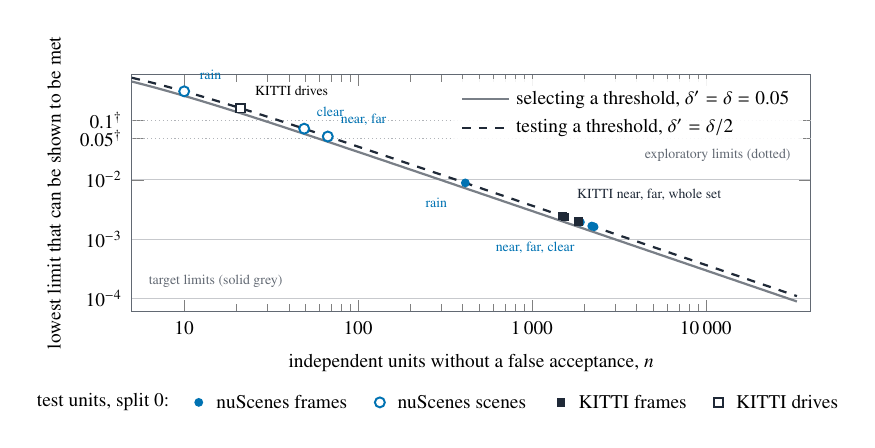
\begin{tikzpicture}
\begin{axis}[width=10.2cm, height=4.6cm,
  xmode=log, ymode=log, xmin=5, xmax=40000, ymin=6e-5, ymax=0.6,
  xlabel={independent units without a false acceptance, $n$},
  ylabel={lowest limit that can be shown to be met},
  tick label style={font=\scriptsize}, label style={font=\scriptsize},
  axis line style={ink!70}, clip=false,
  xtick={10,100,1000,10000}, xticklabels={10,100,1\,000,10\,000},
  ytick={1e-4,1e-3,1e-2,0.05,0.1}, yticklabels={$10^{-4}$,$10^{-3}$,$10^{-2}$,0.05\expl,0.1\expl},
  legend style={font=\scriptsize, draw=none, fill=white, fill opacity=0.9, text opacity=1, at={(0.99,0.98)}, anchor=north east},
  legend cell align=left]
  \draw[ink!25, line width=0.4pt] (axis cs:5,1e-4) -- (axis cs:40000,1e-4);
  \draw[ink!25, line width=0.4pt] (axis cs:5,1e-3) -- (axis cs:40000,1e-3);
  \draw[ink!25, line width=0.4pt] (axis cs:5,1e-2) -- (axis cs:40000,1e-2);
  \draw[ink!35, line width=0.4pt, densely dotted] (axis cs:5,0.05) -- (axis cs:40000,0.05);
  \draw[ink!35, line width=0.4pt, densely dotted] (axis cs:5,0.1) -- (axis cs:40000,0.1);
  \addplot[ink!60, line width=0.8pt] coordinates {(5,0.45072) (5.296,0.431998) (5.61,0.413739) (5.943,0.395962) (6.295,0.378686) (6.668,0.361923) (7.063,0.345683) (7.481,0.329972) (7.924,0.314794) (8.394,0.30015) (8.891,0.286037) (9.418,0.272454) (9.976,0.259393) (10.57,0.246847) (11.19,0.234808) (11.86,0.223266) (12.56,0.212211) (13.3,0.201629) (14.09,0.191509) (14.93,0.181837) (15.81,0.1726) (16.75,0.163784) (17.74,0.155375) (18.79,0.147359) (19.91,0.139721) (21.08,0.132448) (22.33,0.125526) (23.66,0.118939) (25.06,0.112676) (26.54,0.106723) (28.12,0.101065) (29.78,0.0956917) (31.55,0.0905892) (33.42,0.0857456) (35.4,0.0811494) (37.49,0.076789) (39.72,0.0726536) (42.07,0.0687325) (44.56,0.0650155) (47.2,0.0614929) (50,0.0581551) (52.96,0.0549931) (56.1,0.0519983) (59.43,0.0491623) (62.95,0.0464772) (66.68,0.0439353) (70.63,0.0415293) (74.81,0.0392524) (79.24,0.0370979) (83.94,0.0350595) (88.91,0.0331312) (94.18,0.0313072) (99.76,0.0295821) (105.7,0.0279506) (111.9,0.0264079) (118.6,0.0249493) (125.6,0.0235702) (133,0.0222665) (140.9,0.0210341) (149.3,0.0198693) (158.1,0.0187683) (167.5,0.0177278) (177.4,0.0167445) (187.9,0.0158152) (199.1,0.0149372) (210.8,0.0141075) (223.3,0.0133237) (236.6,0.0125831) (250.6,0.0118834) (265.4,0.0112224) (281.2,0.0105979) (297.8,0.0100081) (315.5,0.00945089) (334.2,0.00892458) (354,0.00842746) (374.9,0.00795791) (397.2,0.00751443) (420.7,0.00709558) (445.6,0.00669999) (472,0.00632638) (500,0.00597355) (529.6,0.00564034) (561,0.00532567) (594.3,0.0050285) (629.5,0.00474788) (666.8,0.00448289) (706.3,0.00423265) (748.1,0.00399635) (792.4,0.00377322) (839.4,0.00356253) (889.1,0.00336358) (941.8,0.00317572) (997.6,0.00299834) (1057,0.00283085) (1119,0.00267271) (1186,0.00252339) (1256,0.0023824) (1330,0.00224928) (1409,0.00212359) (1493,0.00200492) (1581,0.00189287) (1675,0.00178708) (1774,0.0016872) (1879,0.00159289) (1991,0.00150386) (2108,0.00141979) (2233,0.00134042) (2366,0.00126549) (2506,0.00119474) (2654,0.00112795) (2812,0.00106488) (2978,0.00100534) (3155,0.000949132) (3342,0.000896063) (3540,0.000845959) (3749,0.000798656) (3972,0.000753996) (4207,0.000711833) (4456,0.000672027) (4720,0.000634447) (5000,0.000598967) (5296,0.000565471) (5610,0.000533847) (5943,0.000503992) (6295,0.000475806) (6668,0.000449196) (7063,0.000424073) (7481,0.000400356) (7924,0.000377964) (8394,0.000356825) (8891,0.000336868) (9418,0.000318027) (9976,0.000300239) (1.057e+04,0.000283447) (1.119e+04,0.000267593) (1.186e+04,0.000252626) (1.256e+04,0.000238496) (1.33e+04,0.000225156) (1.409e+04,0.000212563) (1.493e+04,0.000200673) (1.581e+04,0.000189449) (1.675e+04,0.000178852) (1.774e+04,0.000168848) (1.879e+04,0.000159404) (1.991e+04,0.000150487) (2.108e+04,0.00014207) (2.233e+04,0.000134123) (2.366e+04,0.000126621) (2.506e+04,0.000119538) (2.654e+04,0.000112852) (2.812e+04,0.000106539) (2.978e+04,0.00010058) (3.155e+04,9.49538e-05) (3.342e+04,8.96424e-05)};
  \addlegendentry{selecting a threshold, $\delta'=\delta=0.05$}
  \addplot[ink, line width=0.8pt, dashed] coordinates {(5,0.521824) (5.296,0.501676) (5.61,0.481877) (5.943,0.462465) (6.295,0.443471) (6.668,0.424924) (7.063,0.406848) (7.481,0.389262) (7.924,0.372182) (8.394,0.355619) (8.891,0.339582) (9.418,0.324075) (9.976,0.309103) (10.57,0.294663) (11.19,0.280754) (11.86,0.267372) (12.56,0.25451) (13.3,0.242161) (14.09,0.230314) (14.93,0.21896) (15.81,0.208088) (16.75,0.197685) (17.74,0.187739) (18.79,0.178236) (19.91,0.169162) (21.08,0.160505) (22.33,0.152248) (23.66,0.144379) (25.06,0.136884) (26.54,0.129747) (28.12,0.122955) (29.78,0.116495) (31.55,0.110352) (33.42,0.104514) (35.4,0.0989672) (37.49,0.0936992) (39.72,0.0886976) (42.07,0.0839505) (44.56,0.0794462) (47.2,0.0751736) (50,0.0711217) (52.96,0.0672803) (56.1,0.0636391) (59.43,0.0601886) (62.95,0.0569195) (66.68,0.0538228) (70.63,0.05089) (74.81,0.0481129) (79.24,0.0454837) (83.94,0.0429949) (88.91,0.0406393) (94.18,0.0384102) (99.76,0.0363011) (105.7,0.0343057) (111.9,0.0324181) (118.6,0.0306328) (125.6,0.0289442) (133,0.0273475) (140.9,0.0258376) (149.3,0.0244101) (158.1,0.0230605) (167.5,0.0217846) (177.4,0.0205787) (187.9,0.0194388) (199.1,0.0183614) (210.8,0.0173433) (223.3,0.0163811) (236.6,0.0154719) (250.6,0.0146127) (265.4,0.013801) (281.2,0.013034) (297.8,0.0123094) (315.5,0.0116249) (334.2,0.0109782) (354,0.0103672) (374.9,0.00979016) (397.2,0.00924505) (420.7,0.00873015) (445.6,0.00824381) (472,0.00778446) (500,0.00735061) (529.6,0.00694085) (561,0.00655386) (594.3,0.00618838) (629.5,0.00584322) (666.8,0.00551726) (706.3,0.00520944) (748.1,0.00491874) (792.4,0.00464423) (839.4,0.00438501) (889.1,0.00414022) (941.8,0.00390908) (997.6,0.00369081) (1057,0.00348471) (1119,0.0032901) (1186,0.00310634) (1256,0.00293283) (1330,0.002769) (1409,0.0026143) (1493,0.00246824) (1581,0.00233033) (1675,0.00220012) (1774,0.00207717) (1879,0.00196109) (1991,0.00185149) (2108,0.00174801) (2233,0.00165031) (2366,0.00155807) (2506,0.00147097) (2654,0.00138875) (2812,0.00131111) (2978,0.00123781) (3155,0.00116861) (3342,0.00110328) (3540,0.00104159) (3749,0.000983356) (3972,0.000928374) (4207,0.000876464) (4456,0.000827456) (4720,0.000781187) (5000,0.000737504) (5296,0.000696263) (5610,0.000657327) (5943,0.000620568) (6295,0.000585865) (6668,0.000553101) (7063,0.000522169) (7481,0.000492966) (7924,0.000465397) (8394,0.000439369) (8891,0.000414796) (9418,0.000391597) (9976,0.000369696) (1.057e+04,0.000349019) (1.119e+04,0.000329498) (1.186e+04,0.000311069) (1.256e+04,0.000293671) (1.33e+04,0.000277245) (1.409e+04,0.000261739) (1.493e+04,0.000247099) (1.581e+04,0.000233278) (1.675e+04,0.00022023) (1.774e+04,0.000207912) (1.879e+04,0.000196283) (1.991e+04,0.000185304) (2.108e+04,0.000174939) (2.233e+04,0.000165154) (2.366e+04,0.000155916) (2.506e+04,0.000147195) (2.654e+04,0.000138961) (2.812e+04,0.000131189) (2.978e+04,0.00012385) (3.155e+04,0.000116923) (3.342e+04,0.000110383)};
  \addlegendentry{testing a threshold, $\delta'=\delta/2$}
  \fill[corr] (axis cs:2209,0.00166854) circle (1.6pt);
  \fill[corr] (axis cs:2276,0.00161946) circle (1.6pt);
  \fill[corr] (axis cs:1900,0.00193963) circle (1.6pt);
  \fill[corr] (axis cs:414,0.00887076) circle (1.6pt);
  \filldraw[fill=white, draw=corr, line width=0.7pt] (axis cs:67,0.0535697) circle (1.8pt);
  \filldraw[fill=white, draw=corr, line width=0.7pt] (axis cs:49,0.0725193) circle (1.8pt);
  \filldraw[fill=white, draw=corr, line width=0.7pt] (axis cs:10,0.308497) circle (1.8pt);
  \fill[ink] (axis cs:1500,0.00245623) ++(-1.5pt,-1.5pt) rectangle ++(3pt,3pt);
  \fill[ink] (axis cs:1545,0.00238478) ++(-1.5pt,-1.5pt) rectangle ++(3pt,3pt);
  \fill[ink] (axis cs:1852,0.00198985) ++(-1.5pt,-1.5pt) rectangle ++(3pt,3pt);
  \node[font=\tiny, text=corr, anchor=north east] at (axis cs:2000,0.00132) {near, far, clear};
  \node[font=\tiny, text=corr, anchor=north east] at (axis cs:370,0.0071) {rain};
  \node[font=\tiny, anchor=south west, text=ink] at (axis cs:1600,0.0031) {KITTI near, far, whole set};
  \node[font=\tiny, text=corr, anchor=south west] at (axis cs:70,0.057) {near, far};
  \node[font=\tiny, text=corr, anchor=south west] at (axis cs:51,0.079) {clear};
  \node[font=\tiny, text=corr, anchor=south west] at (axis cs:10.8,0.335) {rain};
  \node[font=\tiny, text=ink!70, anchor=south west] at (axis cs:5.5,1.05e-4) {target limits (solid grey)};
  \node[font=\tiny, text=ink!70, anchor=north east] at (axis cs:3.5e4,0.048) {exploratory limits (dotted)};
  \draw[ink, line width=0.7pt, fill=white] (axis cs:21,0.161098) ++(-1.6pt,-1.6pt) rectangle ++(3.2pt,3.2pt);
  \node[font=\tiny, anchor=south west] at (axis cs:22.5,0.178) {KITTI drives};
\end{axis}
\begin{scope}[shift={(0.6,-1.15)}]
  \node[font=\scriptsize, anchor=east] at (0,0) {test units, split 0:};
  \fill[corr] (0.25,0) circle (1.6pt); \node[font=\scriptsize, anchor=west] at (0.35,0) {nuScenes frames};
  \filldraw[fill=white, draw=corr, line width=0.7pt] (2.55,0) circle (1.8pt); \node[font=\scriptsize, anchor=west] at (2.65,0) {nuScenes scenes};
  \fill[ink] (4.85,0) ++(-1.5pt,-1.5pt) rectangle ++(3pt,3pt); \node[font=\scriptsize, anchor=west] at (4.95,0) {KITTI frames};
  \draw[ink, line width=0.7pt, fill=white] (6.85,0) ++(-1.6pt,-1.6pt) rectangle ++(3.2pt,3.2pt); \node[font=\scriptsize, anchor=west] at (6.95,0) {KITTI drives};
\end{scope}
\end{tikzpicture}
\end{document}
